\documentclass[10pt]{exam}

\usepackage{amssymb, amsmath, amsthm, mathrsfs, multicol, graphicx} 
\usepackage{tikz}

\def\d{\displaystyle}
\def\?{\reflectbox{?}}
\def\b#1{\mathbf{#1}}
\def\f#1{\mathfrak #1}
\def\c#1{\mathcal #1}
\def\s#1{\mathscr #1}
\def\r#1{\mathrm{#1}}
\def\N{\mathbb N}
\def\Z{\mathbb Z}
\def\Q{\mathbb Q}
\def\R{\mathbb R}
\def\C{\mathbb C}
\def\F{\mathbb F}
\def\A{\mathbb A}
\def\X{\mathbb X}
\def\E{\mathbb E}
\def\O{\mathbb O}
\def\pow{\mathscr P}
\def\inv{^{-1}}
\def\nrml{\triangleleft}
\def\st{:}
\def\~{\widetilde}
\def\rem{\mathcal R}
\def\iff{\leftrightarrow}
\def\Iff{\Leftrightarrow}
\def\and{\wedge}
\def\And{\bigwedge}
\def\AAnd{\d\bigwedge\mkern-18mu\bigwedge}
\def\Vee{\bigvee}
\def\VVee{\d\Vee\mkern-18mu\Vee}
\def\imp{\rightarrow}
\def\Imp{\Rightarrow}
\def\Fi{\Leftarrow}

\def\={\equiv}
\def\var{\mbox{var}}
\def\mod{\mbox{Mod}}
\def\Th{\mbox{Th}}
\def\sat{\mbox{Sat}}
\def\con{\mbox{Con}}
\def\bmodels{=\joinrel\mathrel|}
\def\iffmodels{\bmodels\models}
\def\dbland{\bigwedge \!\!\bigwedge}
\def\dom{\mbox{dom}}
\def\rng{\mbox{range}}
\DeclareMathOperator{\wgt}{wgt}

\def\circleA{(-.5,0) circle (1)}
\def\circleAlabel{(-1.5,.6) node[above]{$A$}}
\def\circleB{(.5,0) circle (1)}
\def\circleBlabel{(1.5,.6) node[above]{$B$}}
\def\circleC{(0,-1) circle (1)}
\def\circleClabel{(.5,-2) node[right]{$C$}}
\def\twosetbox{(-2,-1.5) rectangle (2,1.5)}
\def\threesetbox{(-2,-2.5) rectangle (2,1.5)}


\def\bar{\overline}

%\pointname{pts}
\pointsinmargin
\marginpointname{pts}
\marginbonuspointname{pts-bns}
\addpoints
\pagestyle{head}
%\printanswers

\firstpageheader{Math 228}{\bf Homework 10}{Due: Wednesday, April 15}

\def\vertexsize{4pt}
\newcommand{\vtx}[2]{node[fill,circle,inner sep=0pt, minimum size=\vertexsize,label=#1:#2]{}}
\newcommand{\va}[1]{\vtx{above}{#1}}
\newcommand{\vb}[1]{\vtx{below}{#1}}
\newcommand{\vr}[1]{\vtx{right}{#1}}
\newcommand{\vl}[1]{\vtx{left}{#1}}
\renewcommand{\v}{\vtx{above}{}}

\begin{document}
\noindent \textbf{Instructions}: Same rules as usual - turn in your work on separate sheets of paper.  You must justify all your answers for full credit.

\begin{questions}

\question[6] Consider the following two graphs:\\
$G_1$: $V_1=\{a,b,c,d,e,f,g\}$, $E_1=\{\{a,b\},\{a,d\},\{b,c\},\{b,d\},\{b,e\},\{b,f\},\{c,g\},\{d,e\},\{e,f\},\{f,g\}\}$.\\
$G_2$: $V_2=\{v_1,v_2,v_3,v_4,v_5,v_6,v_7\}$, \\$E_2=\{\{v_1,v_4\},\{v_1,v_5\},\{v_1,v_7\},\{v_2,v_3\},\{v_2,v_6\},\{v_3,v_5\},\{v_3,v_7\},\{v_4,v_5\},\{v_5,v_6\},\{v_5,v_7\}\}$\\
\begin{parts}
\part Let $f:G_1 \rightarrow G_2$ be a function that takes the vertices of Graph 1 to vertices of Graph 2.  The function is given by the following table:

\begin{center}
\begin{tabular}{c*{7}{|c}}
$x$ & $a$ & $b$ & $c$ & $d$ & $e$ & $f$ & $g$ \\ \hline
$f(x)$ & $v_4$ & $v_5$ & $v_1$ & $v_6$ & $v_2$ & $v_3$ & $v_7$ 
\end{tabular}
\end{center}
%
%\[f(a)=v_4\]
%\[f(b)=v_5\]
%\[f(c)=v_1\]
%\[f(d)=v_6\]
%\[f(e)=v_2\]
%\[f(f)=v_3\]
%\[f(g)=v_7\]
Does $f$ define an isomorphism between Graph 1 and Graph 2? Explain.
\begin{solution}
Recall that in order for $f$ to define an isomorphism between $G1$ and $G2$, it must preserve relationships between vertices. To put this into context, this means that since $a$ and $b$ are joined via an edge in $G1$ that their corresponding vertices in $G2$ must also be joined by an edge. This must be true for all of the vertices and edges. When examining the function, we can see that the vertex $g$ goes to $v_7$, that is $f(g)=v_7$. BUT, $g$ has exactly 2 edges (so $g$ is degree 2) and $v_7$ is degree 3. This means that $f$ cannot possibly be an isomorphism. Similarly, we can see that $f$ does not take $c$ to the correct vertex either $c$ is degree 2 and $v_1$ has degree 3. 
\end{solution}
\part Define a new function $g$ (with $g\not=f$) that defines an isomorphism between Graph 1 and Graph 2.
\begin{solution}
\begin{center}
\begin{tabular}{c*{7}{|c}}
$x$ & $a$ & $b$ & $c$ & $d$ & $e$ & $f$ & $g$ \\ \hline
$f(x)$ & $v_4$ & $v_5$ & $v_6$ & $v_1$ & $v_7$ & $v_3$ & $v_2$ 
\end{tabular}
\end{center}
\end{solution}
\part Is the graph pictured below isomorphic to Graph 1 and Graph 2? Explain.
\begin{center}
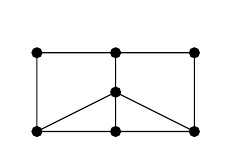
\begin{tikzpicture}
\draw (-1, 0) coordinate (v1) -- (0,0) coordinate (v2) -- (1,0) coordinate (v3) -- (1,1) coordinate (v4) -- (0,1) coordinate (v5) -- (-1,1) coordinate (v6) -- (v1) --(0,.5) coordinate (v7) -- (v2) (v7) -- (v3) (v7) -- (v5);
\foreach \i in {1,...,7}{
	\fill (v\i) \v;
} 
\end{tikzpicture}
\begin{solution}
No, it could not possibly be isomorphic. If you count up the degrees of each vertex in this picture, you can see that the highest degree is 4 (the center vertex). In order to be isomorphic to either $G1$ or $G2$ we would definitely need a vertex of degree 5, which we don't have.
\end{solution}

\end{center}

\end{parts}



\question[9] Recall that in class we proved that every (connected) planar graph with $V$ vertices, $E$ edges and $F$ faces satisfied $V - E + F = 2$.  We also saw that every convex polyhedron could be represented as a planar graph.
\begin{parts}
\part An {\em octahedron} is a regular polyhedron made up of 8 equilateral triangles (it sort of looks like two pyramids with their bases glued together).  Draw a planar graph representation of an octahedron.  How many vertices, edges and faces does an octahedron (and your graph) have?
\begin{solution}
Since there are 8 triangles, there must be 8 faces.  We can count the number of edges by taking $8 \cdot 3 = 24$, but this is double counting since each edge corresponds to two faces.  Thus there are 12 edges.  We can use Euler's formula to find that there are 6 vertices (and this shows that each vertex is the joining of 4 triangles).

The planar representation of the graph is:



\begin{center}
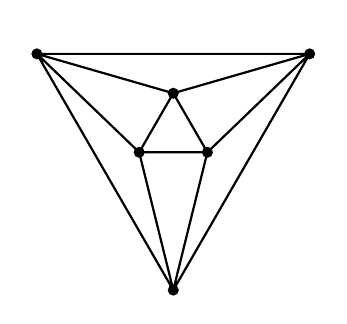
\begin{tikzpicture}
\coordinate (a) at (30:2);
\coordinate (b) at (150:2);
\coordinate (c) at (270:2);
\coordinate (d) at (90:.5);
\coordinate (e) at (210:.5);
\coordinate (f) at (-30:.5);
\draw[thick] (a) \v -- (b) \v -- (c) \v -- (a) -- (d)\v --(e)\v -- (f)\v --(d) -- (b) -- (e) -- (c) -- (f) -- (a);

\end{tikzpicture}
\end{center}


\end{solution}
\part The traditional design of a soccer ball is in fact a (spherical projection of a) truncated icosahedron.  This consists of 12 regular pentagons and 20 regular hexagons.  No two pentagons are adjacent (so the edges of each pentagon are shared only by hexagons).  How many vertices, edges, and faces does a truncated icosahedron have?  Explain how you arrived at your answers.  Bonus: draw the planar graph representation of the truncated icosahedron.
\begin{solution}
Well, right off we know that the truncated icosahedron has $12+20=32$ faces by counting the number of pentagons and hexagons. Now, because we know that every connected planar graph with $V$ vertices, $E$ edges and $F$ faces satisfied $V - E + F = 2$, we only really need to find out the number of edges or the number of vertices since $V-E=-30$. So, let's maybe try to figure out the number of edges we have. If we think about the number of total edges when the pentagons and hexagons are not attached, we know that we have $5\times 12+6\times 20=180$. But each of these edges is shared with another edge, which means that we have cut the number of edges in half. So, we have $90$ edges, which then gives us $60$ vertices.
\end{solution}
\part Your ``friend'' claims that he has constructed a convex polyhedron out of 2 triangles, 2 squares, 6 pentagons and 5 octagons.  Prove that your friend is lying.  Hint: each vertex of a convex polyhedron must border at least three faces.
\begin{solution}
So, let's assume for a contradiction that your friend really has constructed a convex polyhedron. Then, we would know that the polyhedron has $15$ faces, $(2\times 3+2\times 4+6\times 5+5\times 8)/2 = 42$ edges, and $V=2+42-15=29$ vertices. Now, using the hint, we also know that $3V\leq F$ but $3\times 29$ is not in fact less than $15$. So we have a contradiction, and your friend is lying.
\end{solution}
\end{parts}

\question[6] Prove that the {\em Petersen graph} (below) is not planar.  Hint: what is the length of the shortest cycle?

\begin{center}
  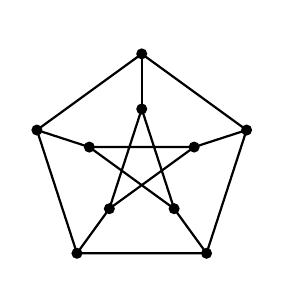
\begin{tikzpicture}[scale=.7]
    \draw[thick] (18:2) -- (90:2) -- (162:2)  -- (234:2) -- (306:2) -- cycle; 
    \draw[thick] (18:1) --  (162:1)  -- (306:1) -- (90:1) -- (234:1) --cycle;
    \foreach \x in {18, 90, 162, 234, 306}
    \draw[thick] (\x:1) \v -- (\x:2) \v;
  \end{tikzpicture}
\end{center}

\begin{solution}
  \begin{proof}
    Suppose, for contradiction, that the Petersen graph were planar.  Then it would satisfy Euler's formula: $V - E + F = 2$.  Since the graph has 10 vertices and 15 edges, this says that there must be $7$ faces.  
    
    Now let $B$ be the total number of boundaries around all faces when the graph is drawn in a planar way.  Since each edge is used in two boundaries we have $B = 2E$.  On the other hand, each face is surrounded by {\em at least} 5 boundaries, since the shortest cycle (circuit) in the graph contains 5 edges.  Thus $F \le \frac{B}{5}$.  Putting these two facts together we get
    \[F \le \frac{2E}{5}\]
    This is a contradiction, since $7 \not\le \frac{2\cdot 30}{6}$.  Alternatively, the above relationship says that $F \le 6$, but we said $F = 7$ above.
    
    Therefore the Petersen graph is not planar.
  \end{proof}

\end{solution}


\question[9] Remember that a {\em tree} is a connected graph with no cycles.
\begin{parts}
\part Conjecture a relationship between a tree graph's vertices and edges. (For instance, can you have a tree with 5 vertices and 7 edges?)
\begin{solution}
After drawing a few trees, you should notice that there is always exactly one more vertices than edges. That is $V=E+1$
\end{solution}
\part Explain why every tree with at least 3 vertices has a leaf (i.e., a vertex of degree 1). 
\begin{solution}
Assume for a contradiction that every tree with at least 3 vertices does not have a leaf. Namely, that there are no vertices of degree 1. Then, every vertex must have a degree of 2 or more, but this would imply that we have a cycle! Why? Think about taking a path from one vertex to another. Choose the first vertex and a route to leave it (remember it should have at least two ways to leave). Once I leave that vertex I reach another vertex which also has at least one more way to leave. Keep doing this. Eventually you will get back to one of the vertices that you have already visited and therefore you will have completed a cycle. 
\end{solution}
\part Prove your conjecture from part (a) by induction on the number of vertices. Hint: For the inductive step, you will assume that your conjecture is true for all trees with $k$ vertices, and show it is also true for an arbitrary tree with $k+1$ vertices.  Consider what happens when you cut off a leaf and then let it regrow.
\begin{solution}
Recall that we need two parts for an induction proof: a base case and an inductive case.
\begin{proof}
Let $P(n)$ be the statement ``a tree graph $T_n$ with $n$ vertices has $n-1$ edges.
Base Case: Draw a tree with three vertices. Clearly you have only 2 edges (otherwise you would have a cycle).\\
Inductive Case: Assume $P(k)$ is true for some arbitrary $3<k<n$.\\
NTS: $P(k+1)$ is true. That is $T_{k+1}$ has $k$ edges.\\
Let $T_{k+1}$ be a tree graph with $k+1$ vertices. By part (b) we know that every tree with at least 3 vertices has a leaf, so cut that one leaf off of $T_{k+1}$. Then our tree graph has only $k$ vertices, and by our inductive case has $k-1$ edges. Well, if we let that leaf regrow we will add both one edge and one vertex, which means that we will have a tree graph with $k+1$ vertices and $k-1+1=k$ edges. TBTPOMI we have shown that $P(n)$ is true.


\end{proof}
\end{solution}
\end{parts}


%\question Edward A. Mouse has just finished his brand new house.  The floor plan is shown below:
%
%\begin{center}
%  \begin{tikzpicture}[scale=.8]
%    \draw[very thick] (-3,0) rectangle (3,3);
%    \draw[very thick] (-3,1.8) --(-2.7,1.8) (-2.3,1.8) -- (-1.5, 1.8) (-1.5, 1.6) -- (-1,1.6) (-.6, 1.6) -- (.3,1.6) (.7,1.6) -- (1, 1.6) (1, .8) -- (1.5, .8) (1.9,.8) -- (3,.8); 
%    \draw[very thick] (-1.5,0) -- (-1.5, .8) (-1.5, 1.2) -- (-1.5,2.1) (-1.5,2.5) -- (-1.5,3);
%    \draw[very thick] (0,0) -- (0,.6) (0,1) -- (0,1.6);
%    \draw[very thick] (1,0) -- (1,.2) (1,.6) -- (1,1) (1,1.4) -- (1,2.1) (1,2.5) -- (1,3);
%  \end{tikzpicture}
%\end{center}
%
%
%\begin{parts}
% \part[3] Edward wants to give a tour of his new pad to a lady-mouse-friend.  Is it possible for them to walk through every doorway exactly once?  If so, in which rooms must they begin and end the tour? Explain.
% \begin{solution}
%   Yes, he must start in the top right room and end in the bottom middle room, or vice versa.  This is because those are the two rooms with an odd number of doors.  
%   
%   In graph theory terms, if we place a vertex in each room and connect vertices if there is a door between their rooms, we are asking whether the graph has an Euler path.  The number of doors is the degree of the vertex, and a graph has an Euler path if and only if there are two or fewer vertices with odd degree.  In that case, the path must start at one of those odd degree vertices and end at the other.
% \end{solution}
%
%\part[2] Is it possible to tour the house visiting each room exactly once?  Explain.
%
%\begin{solution}
%  Yes.  This does not correspond to an Euler path or circuit, since all we need to do is visit each vertex exactly once.  It is easy to do - for example, tour the house clockwise.
%\end{solution}
%
%
%\part[3] After a few mouse-years, Edward decides to remodel.  He would like to add some new doors between the rooms he has.  Of course, he cannot add any doors to the exterior of the house.  Is it possible for each room to have an odd number of doors? Explain.
%\begin{solution}
%  No it is not possible.  If each room had an odd number of doors, then the corresponding graph would have the property that the degree of every vertex would be odd.  There are 7 vertices, and if their degrees were all odd, then the sum of the degrees would be an odd number as well.  But the number of edges in a graph is always 1/2 the sum of the degrees, so the sum of the degrees must be even.
%  
%  In other words, if you add up the number of doors in all rooms, you need to get an even number, since the number of doorways is half this number - each doorway counts as a door in two rooms.
%\end{solution}
%
%\end{parts}


%\question A group of 10 friends decides to head up to a cabin in the woods (where nothing could possibly go wrong).  Unfortunately, a number of these friends have dated each other in the past, and things are still a little awkward.  To get the cabin, they need to divide up into some number of cars, and no two people who dated should be in the same car.
%\begin{parts}
%  \part[3] What is the smallest number of cars you need if all the relationships were strictly heterosexual?  Represent an example of such a situation with a graph.  What kind of graph do you get?
%  \begin{solution}
%    2 cars are needed.  Since no boys dated boys and no girls dated girls, it is possible to separate the youths into cars by gender.  The corresponding graph (with vertices representing people and edges representing the fact that those people dated) would be bipartite - there are no edges between two boys and no edges between two girls.  
%  \end{solution}

%  \part[3] What is the smallest number of cars you need if the relationships could be represented by the Petersen graph (above)?  Assume each person is represented by a vertex, and two people have dated if there is an edge between their vertices. Explain.
%  
%  \begin{solution}
%    3 cars are needed.  The Petersen graph is not bipartite, so 2 cars is not enough.  You can see this because there is an odd circuit.  It is not too difficult to assign vertices to cars (i.e., color the vertices) so that no two adjacent vertices are assigned the same car (color).    
%  \end{solution}
%
%  \part[2] What do these questions have to do with coloring? 
%  \begin{solution}
%    We are really asking for the chromatic number of the graphs.  The smallest number of cars needed is the smallest number of colors needed for a proper vertex coloring.
%  \end{solution}

%\end{parts}

%\question[6] We say that a graph has a {\em Hamilton path} if there is a path which visits each vertex exactly once (you do not need to use every edge in the path).  
%\begin{parts}
%  \part Suppose a graph has a Hamilton path.  What is the maximum number of vertices of degree one the graph can have?  Explain why your answer is correct.
%
%  \begin{solution}
%    Note that a vertex of degree one can only be the start or the end of a Hamilton path - if we go {\em to} a vertex of degree one, we are stuck there - we cannot use the same edge to leave the vertex, because doing so would bring us back to a vertex we have already visited.  If a graph has a Hamilton path, it might start at a vertex of degree one, end at a vertex of degree one, but there cannot be any other vertices of degree one.  Therefore a graph with a Hamilton path can have at most two vertices of degree one.
%  \end{solution}
%
%  \part Find a graph which does not have a Hamilton path even though no vertex has degree one.  Explain why your example works.
%  
%  \begin{solution}
%    There are many such graphs.  Here are two examples:
%    
%    \begin{center}
%      \begin{tikzpicture}
%        \draw[thick] (-1,0) \v -- (0,1) \v -- (1, 0) \v -- (0, .33) \v -- (-1,0) -- (0,-.33) \v -- (1,0) -- (0,-1) \v -- (-1,0);
%      \end{tikzpicture}
%      \hspace{1in}
%      \begin{tikzpicture}
%        \draw[thick] (270:.5) \v -- (255:1) \v -- (285:1) \v -- (270:.5) -- (0,0) \v -- (135:.5) \v -- (150:1) \v -- (120:1) \v -- (135:.5) (0,0) -- (45:.5) \v -- (60:1) \v -- (30:1) \v -- (45:.5);
%      \end{tikzpicture}
%
%    \end{center}
%
%  \end{solution}
%
%\end{parts}


\end{questions}



\end{document}


